\documentclass[submission,copyright,creativecommons]{eptcs}
\providecommand{\event}{SOS 2023} % Name of the event you are submitting to

\usepackage[utf8]{inputenc}
\usepackage[T1]{fontenc}
\usepackage{minted}
\usepackage{hyperref}
\usepackage{amssymb}
\usepackage{amsmath}
\usepackage{tikz}
\usepackage{iftex}
\usepackage{varioref}

\ifpdf
\usepackage{underscore}         % Only needed if you use pdflatex.
\usepackage[T1]{fontenc}        % Recommended with pdflatex
\else
\usepackage{breakurl}           % Not needed if you use pdflatex only.
\fi

\title{Skeletal Semantics of Python}

\author{Martin Andrieux
  \institute{ENS Rennes, France}
  \email{martin.andrieux@ens-rennes.fr}
  \and
  Alan Schmitt
  \institute{Inria, France}
  \email{alan.schmitt@inria.fr}
}

\newcommand{\titlerunning}{A Longtitled Paper}
\newcommand{\authorrunning}{R.J. van Glabbeek, C. Author \& Y.S. Else}

\hypersetup{
  bookmarksnumbered,
  pdftitle    = {\titlerunning},
  pdfauthor   = {\authorrunning},
  pdfsubject  = {EPTCS},               % Consider adding a more appropriate subject or description
  % pdfkeywords = {keyword1, keyword2} % Uncomment and enter keywords specific to your paper
}

\begin{document}
\maketitle

% Will be removed in the future, just for me
\tableofcontents

\begin{abstract}
  We present Pyskel, a formalization of Python semantics in Skel.
  We describe a subset of the Python programming language including assignments,
  function calls, object oriented features and exceptions.
  This formalization can be used to automatically derive interpreters and debuggers.
\end{abstract}

\section{Introduction}\label{sec:introduction}

The Python programming language is widely used by programmers,
but it lacks an official and clear specification, the
\href{https://docs.python.org/3/reference/}{\emph{Python Language Reference}} and
\href{https://docs.python.org/3/library/}{\emph{Python Standard Library}}
begin the closest things to it.

A formal specification of a programming language is necessary to prove properties on programs.
Moreover,

We propose a Skel implementation of Raphaël Monat's Python pure semantics\cite{Monat2021},
as mentionned in~\cite{noizet:hal-03784478}.

\section{Challenges of Python Semantics}
The python semantics, as described in Monat's thesis, is full of mutable state.

\subsection{Scopes}
Python does not have a syntax criteria to distinguish between declarations and assignments. Take a look at the programs figure \vref{fig:scopeillustration}:
\begin{figure}[ht]
  \centering
  \begin{minipage}{0.3\textwidth}
    \begin{minted}{python}

x = 0
def function():

  x = 1
  print(x)

function(); print(x)
    \end{minted}
  \end{minipage}
  \begin{minipage}{0.3\textwidth}
    \begin{minted}{python}

x = 0
def function():
  global x
  x = 1
  print(x)

function(); print(x)
    \end{minted}
  \end{minipage}
  \begin{minipage}{0.3\textwidth}
    \begin{minted}{python}
def wrapper():
  x = 0
  def function():
    nonlocal x
    x = 1
    print(x)

  function(); print(x)
wrapper()
    \end{minted}
  \end{minipage}
  \caption{\label{fig:scopeillustration}Three programs illustrating scopes behavior}
\end{figure}

The first one will output \texttt{1} and \texttt{0}: by default, assignments are declarations.
The first code sample contains to variables named \texttt{x}: the global one (equal to zero), and one local to \texttt{function} (equal to one).

To use the global version of \texttt{x} in \texttt{function}, the \texttt{global} keyword must be used.
This meaning is ``Some variable \texttt{x} is already defined in the global scope, use this one instead of creating a new one''.
The second program will therefore display \texttt{1} and \texttt{1}.

One trickier case is the third program.
It is very close to the second one but with one little difference: the entire code is place in a function (called \texttt{wrapper} in the example).
To use the \texttt{x} variable defined in the \texttt{wrapper} function inside of \texttt{function}, we cannot use the \texttt{global} keyword, because \texttt{x} is not \texttt{global}.
In this case, the \texttt{nonlocal} keyword is what we need.
It uses the closest definition of \texttt{x} among the upper scopes.
Like the second one, it displays two \texttt{1}.

\subsection{Objects and Classes}
Python values are stored on the heap.
They can be
\begin{itemize}
\item builtin constants: such as integers, strings, booleans, \dots.
\item Functions or methods
\item Classes
\item Intances
\end{itemize}

A class defines a new \emph{type}, it can be seen as a set of definitions.
These definitions forms the \emph{fields} of a class.
Programmers familiar with object-oriented programming know that classes can inherit from each other.
The set of all the fields of a class and its superclasses forms the \emph{attributes} of this class.

The notion of field is hidden in python, but it is nevertheless necessary to understand the underlying mechanism of classes.
In the code sample giver figure~\vref{fig:class}, the class \texttt{Example} has three fields: \texttt{value}, \texttt{function} and \texttt{method}.
From the point of vue of the class, nothing distinguish \texttt{function} and \texttt{method} (except the number of arguments).
The self parameter is not a keyword, but an identifier like any other.

\begin{figure}[ht]
  \centering
  \begin{minipage}{0.25\textwidth}
    \begin{minted}{python}
class Example:
  value = 0
  def function():
    return 1

  def method(self):
    self.x = 2
    \end{minted}
  \end{minipage}
  \caption{\label{fig:class}A class in Pyhton}
\end{figure}


An instance is simply a reference to some class.
The question is: where is stored the \texttt{x} of \texttt{Example}'s instances?
Each python object has an additional dictionnary where its dynamic attributes are stored.




\subsection{Internal Functions}


\section{Fundamental Concepts}\label{sec:skel}

\subsection{Evaluation Monad and State}\label{sec:monad}
\subsubsection{Stateful computation}
A python program is represented in Skel by a data structure very close to the Python Abstract Syntax Tree.
Evaluating a python program is therefore equivalent to evaluating a list of statements.
The evaluation takes place in a monad containing the following context:
\begin{itemize}
\item A read-only state, containing the local environment and built-in objects,
\item A read-write state, containing the heap and the scopes,
\item The runtime state: either \texttt{Cur} for a successful computation, or \texttt{Flag}:
  for control flow operations, such as \texttt{Return}, \texttt{Break}, \texttt{Continue}, or \texttt{Exception}.
\end{itemize}
The manipulation of this information is detailed in the following sections.

Writting the evaluator in the monad makes code simpler to understand for multiple reasons.
First, if a function does not use a part of the state, the relevent part will not be visible at all in the function definition
(while in a more classical approach based on argument passing, functions have to take additional parameters and pass them to other functions without modifying them).
Secondly, code can be written in an imperative style.

\subsubsection{State}
To evaluate properly a Python program, we consider the following state.

\begin{itemize}
\item A Heap, mapping from addresses to values,
\item An Environment, containing a scope identifier and a mapping from variable names to either \texttt{Local}, \texttt{Global} or \texttt{NonLocal},
\item A Scope Heap, which maps scope identifiers to scopes
\end{itemize}

\subsubsection{}

\section{Scopes Management}
Scopes are not handled in Monat's thesis, we present an extension of the semantics allowing mutiple scopes in Pyskel.
In the semantics, there is a unique environment \(\mathcal E \overset{\text{def}}{=} \mathsf{Id} \rightharpoonup \mathsf{Addr} \cup \mathtt{LocalUndef}\).
The keywords \texttt{global} and \texttt{nonlocal} are not supported.
Undefined variables are detected at parsing time and illformed programs are not accepted.

\subsection{Scopes in Python}
We expose in this section the main concepts of scope management in Python through a few examples.

First, the \emph{global scope} contains all the toplevel declarations, it is a mapping from varialbe names to heap addresses.
It contains toplevel variables, such as user-defined functions, and builtin objects.

Functions evaluation requires local memory.
This local memory corresponds to a fresh scope containing the function parameter and local variables.

The last type of evaluation context is class definitions.
They behave like function, but without the concept of unbound locals.

\subsubsection{Function body}
By default, each statement of the form \texttt{id = value} will allocate a new variable \texttt{x} in the current scope.
To modify a global variable from the body of a function, one must use the \texttt{global} keyword.
By doing so, assignments to some variable \texttt{x} will effectively modify the global \texttt{x} without creating a local variable in the function body.
To use some variable defined in one of the upper scpoes, but not necesseraly the global one, we use the \texttt{nonlocal} keyword.

To implement the \texttt{global} and \texttt{local} keywords, a function must know the global scope and the scope in wich it was defined.
We depict this dependency as a tree of scope, as shown in figure \vref{fig:functionscope}.

\begin{figure}[ht!]
  \begin{minipage}{0.35\textwidth}
  \begin{minted}{python}
def wrapper():
  data = # some data
  def worker():
    nonlocal data # mandatory
    # work
  return worker()

x = 0
def incr():
  global x
  x = x + 1
  \end{minted}
  \end{minipage}
  \begin{minipage}{0.6\textwidth}
  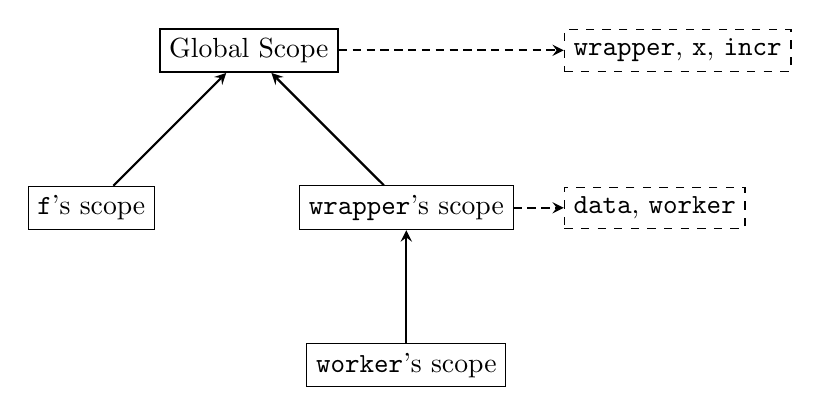
\begin{tikzpicture}
    \node[draw, thick] (GS) at (0, 0) {Global Scope};
    \node[draw] (Wr) at (2, -2) {\texttt{wrapper}'s scope};
    \node[draw] (Wo) at (2, -4) {\texttt{worker}'s scope};
    \node[draw] (F) at (-2, -2) {\texttt{f}'s scope};
    \node[draw, dashed, right] (GSV) at (4, 0) {\texttt{wrapper}, \texttt{x}, \texttt{incr}};
    \node[draw, dashed, right] (WrV) at (4, -2) {\texttt{data}, \texttt{worker}};
    \draw[->, >=stealth, thick] (Wr) to (GS);
    \draw[->, >=stealth, thick] (Wo) to (Wr);
    \draw[->, >=stealth, thick] (F) to (GS);
    \draw[->, >=stealth, densely dashed, thick] (GS) -- (GSV);
    \draw[->, >=stealth, densely dashed, thick] (Wr) -- (WrV);
  \end{tikzpicture}
  \end{minipage}
  \caption{\label{fig:functionscope}Simple functions and the corresponding scopes}
\end{figure}

Note that scopes are computed at parsing time: when a function is called, its local variable are allocated but not initialized yet.
Thus, reading a not yet defined variable in a function definition will result in an \texttt{UnboundLocalError} instead of a classical \texttt{NameError}. This is illustrated figure \vref{fig:unboundlocal}.

\begin{figure}
  \centering
  \begin{minipage}{0.5\textwidth}
  \begin{minted}{python}
def f():
  x = undef # will raise NameError
  x = y     # will raise UnboundLocalError
  y = 0     # because y is local to f
  \end{minted}
  \end{minipage}
  \caption{\label{fig:unboundlocal}Example of a program throwing \texttt{UnboundLocalError}}
\end{figure}

\subsubsection{Classes definition}
Evaluation of classes definition is very close to function evaluations.
The main difference is that variables are \emph{not} allocated before evaluation.

\subsection{Scopes in Pyskel}
In this section, we present how pyskel manages scopes and evaluation contexts.

\subsubsection{Scopes}
Scopes are mutables and potentially references by more than one object.
We use a key-value approach to identify scopes,

As we have seen, classes' scopes and functions' scopes differ in their structure, since functions need to allocate undefined values.
This results in two different scope types in pyskel:
\begin{itemize}
\item total scopes are mapping from identifiers to heap addresses, they are represented by the following type:
  \begin{minted}{sk.py -x}
type total_scope = (tscope_up: maybe<scope_id>, tmapping: map<addr>)
  \end{minted}
  The definition is straight forward, a total scope is a mapping and some optional scope.
  the \texttt{tscope\_up} is used to look up nonlocal variables.
\item partial scopes can accept uninitialized values, we use an option type to represent this property:
  \begin{minted}{sk.py -x}
type maybe<a> =
  | Nothing
  | Just a

type partial_scope = (pscope_up: maybe<scope_id>, pmapping: map<maybe<addr>>)
  \end{minted}
\end{itemize}

Note that scope ids are also useful for the tree structure of the scope. A partial scope can be defined in a total scope and vice versa.

The link betwin scope ids and scopes is done with a map of \texttt{any\_scope}:
\begin{minted}{sk.py -x}
type any_scope = | TotalScope total_scope
                 | PartialScope partial_scope
\end{minted}

\section{Initial State}
As explained Section~\ref{sec:monad}, evaluating a python program is a stateful computation.
Therefore, we need to provide some initial state to the interpreter.
This state must contain builtin objects, such as the two booleans \texttt{true} and \texttt{false}, but also all the builtin classes.

In python all classes inherits from the \texttt{object} class, and are instances of the class type.
The initial state is computed in two steps.
The constants (such as \texttt{None}, \texttt{true} or \texttt{false}) are hardcoded in the semantics.
The builtin classes (such as \texttt{int}, \texttt{BaseException} or \texttt{object}) are defined in a prelude file.

To evaluate a python program, we must evaluate the prelude first, to collect all of its definitions, and then call the evaluator with the output of the prelude on the program file.

\section{Bibliography}
\nocite{*}
\bibliographystyle{eptcs}
\bibliography{paper}
\end{document}

%%% Local Variables:
%%% mode: latex
%%% TeX-command-extra-options: "-shell-escape"
%%% TeX-master: t
%%% End:
